\documentclass[a4paper, 10pt]{article}
\usepackage[utf8]{inputenc}
\usepackage[T1]{fontenc}
\usepackage[french]{babel}
\usepackage{graphicx}
\usepackage{listings}
\usepackage{amssymb}
\usepackage{amsmath}
\usepackage{fullpage}
\usepackage{url}
\usepackage[final]{pdfpages}

\begin{document}
\begin{center}
\section*{Diagramme de Voronoï...}
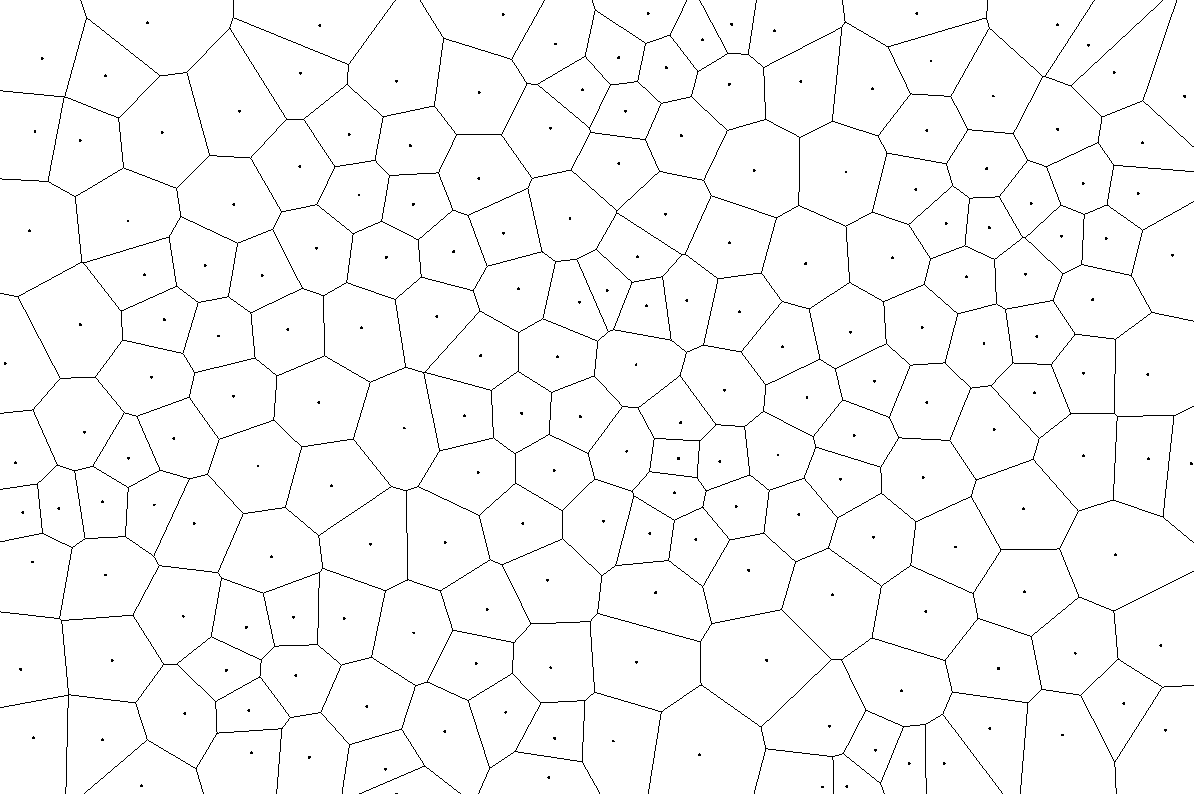
\includegraphics[scale=0.4]{Diagramme200.PNG}
\bigbreak
\bigbreak
\bigbreak
\section*{... et sa triangulation associée !}
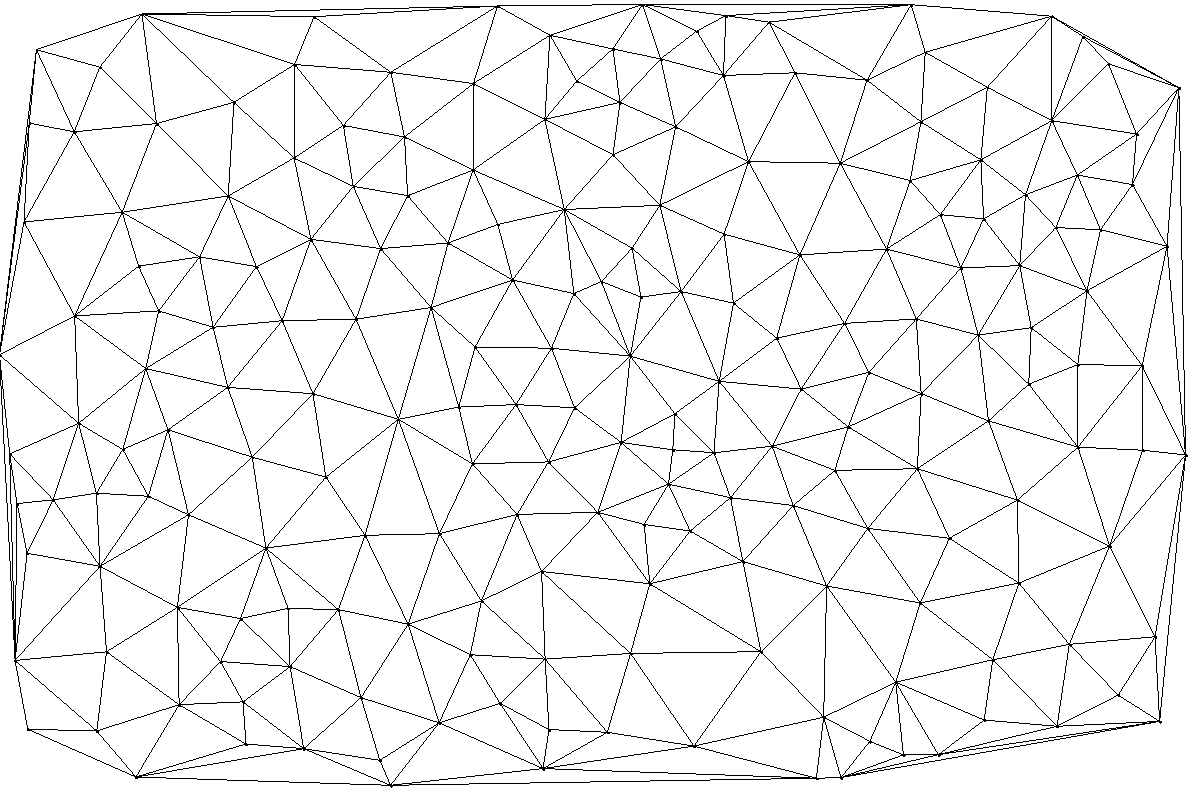
\includegraphics[scale=0.4]{DiagrammeDual200Modifie.PNG}
\end{center} 

\newpage

\begin{center}
\section*{Front parabolique}
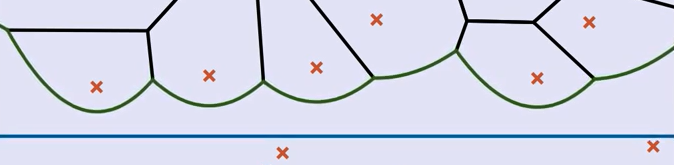
\includegraphics[scale=0.8]{FrontParabolique.PNG}
\bigbreak 
\section*{Évènement Site}  
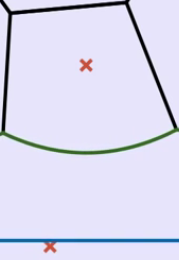
\includegraphics[scale=1]{AvantIntersection.PNG}
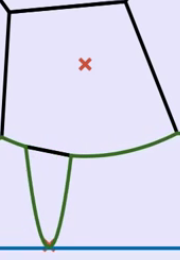
\includegraphics[scale=1]{ApresIntersection.PNG} 
\bigbreak
\section*{Évènement Cercle}  
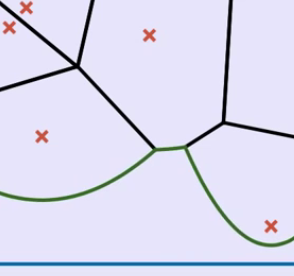
\includegraphics[scale=0.9]{AvantCercle.PNG}
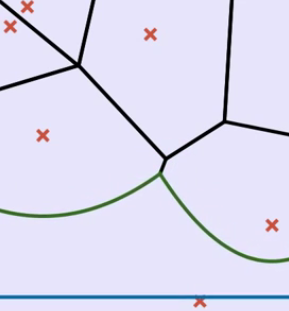
\includegraphics[scale=0.8]{ApresCercle.PNG} 
\bigbreak
\section*{Évènement cercle périmé} 
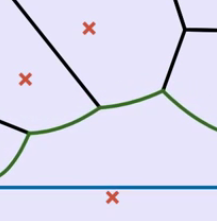
\includegraphics[scale=1]{AvantFauxCercle.PNG}
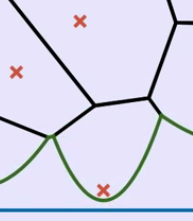
\includegraphics[scale=1]{ApresFauxCercle.PNG}
\bigbreak
\section*{Arbre binaire du front parabolique}
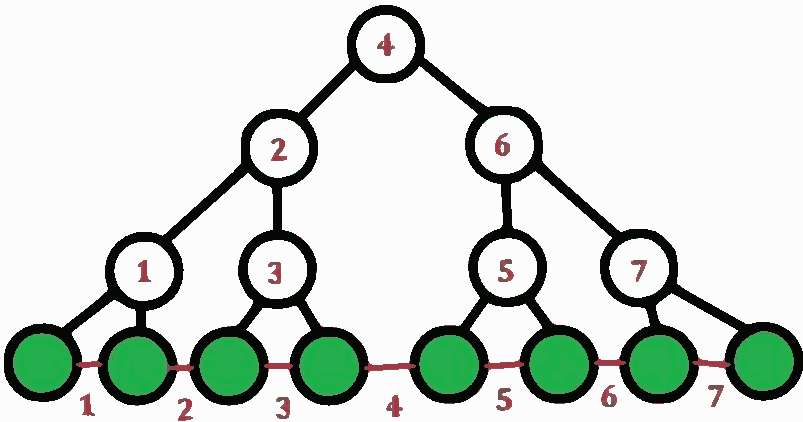
\includegraphics[scale=1]{../Rapport/ArbreBinaire-vect.pdf} 
\end{center}

\newpage

\begin{center}
\section*{Bruit de Perlin}
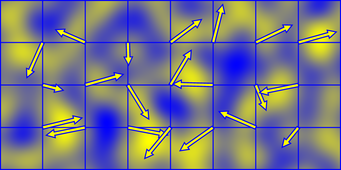
\includegraphics[scale=1]{PerlinNoise.png} 
\end{center}
\begin{center}
\section*{Octaves} 
\end{center}
\begin{flushleft}
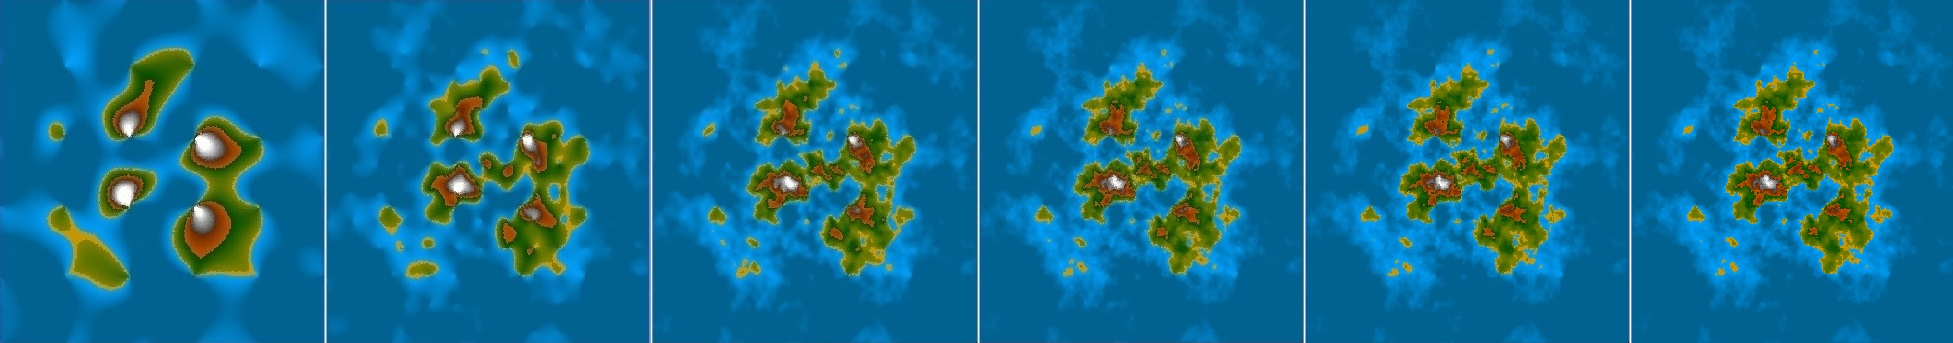
\includegraphics[scale=0.35]{../Rapport/Octaves.jpg} 
\end{flushleft}
\begin{center}
\section*{Île avec gradient de couleur discret} 
\includegraphics[scale=0.4]{island.jpg}  
\bigbreak
\bigbreak
\section*{Île avec gradient de couleur discret} 
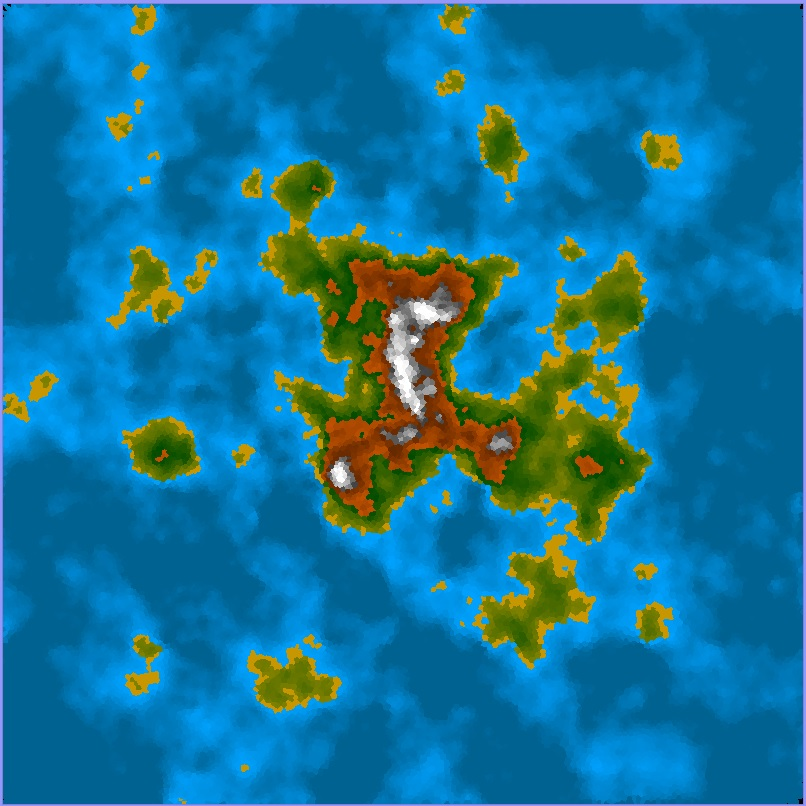
\includegraphics[scale=0.45]{RockyIsland.jpg} 
\bigbreak
\section*{Île avec gradient de couleur continu} 
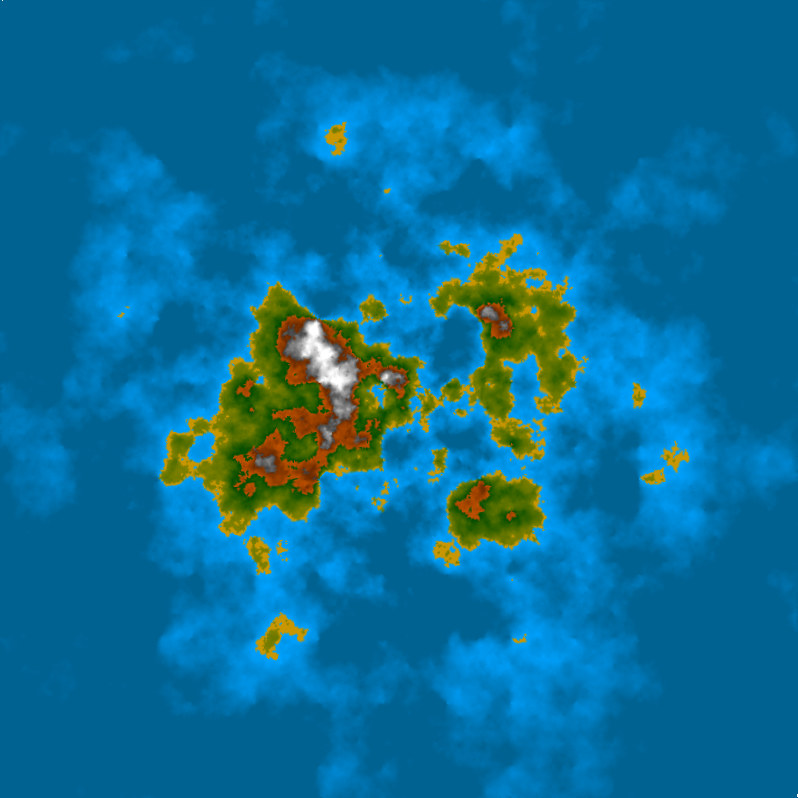
\includegraphics[scale=0.45]{Triangulation.PNG}
\end{center} 
\end{document}
